\documentclass[12 pt]{article}        	%sets the font to 12 pt and says this is an article (as opposed to book or other documents)
\usepackage{amsfonts, amssymb}
\usepackage{amsmath}
\usepackage{mathabx}
\usepackage{graphicx}
\usepackage{esint}
\usepackage{float}

\usepackage[left=2cm,right=2.5cm,top=2cm,bottom=1.5cm]{geometry}

\pagestyle{myheadings}

\newcommand{\eqn}[0]{\begin{array}{rcl}}%begin an aligned equation - allows for aligning = or inequalities.  Always use with $$ $$
\newcommand{\eqnend}[0]{\end{array} }  	%end the aligned equation

\newcommand{\qed}[0]{$\square$}

% personalized commands
\newcommand{\inv}{^{-1}}
\newcommand{\bij}{\mathrlap{\hookrightarrow}\rightarrow}
\newcommand{\onto}{\twoheadrightarrow}
\newcommand{\z}{\mathbb Z}
\newcommand{\real}{\mathbb R}
\newcommand{\q}{\mathbb Q}
\newcommand{\complex}{\mathbb C}
\newcommand{\n}{\mathbb N}
\newcommand{\cont}{\lightning}
\newcommand{\osub}{\stackrel{\circ}{\subset}}

\title{A Faster Attack on LFSR Recurrences}
\begin{document}
\maketitle
\begin{center}
    Timothy Tarter

    Arsenii Herasymov

    Garrett Priebracha

    $\newline$

    James Madison University

    Madison Institute for Mathematical Finance

    https://github.com/Tartertx/LFSR-Research
\end{center}

\begin{abstract}
    Linear Feedback Shift Registers (LFSR) are a type of cryptographic algorithm used to generate pseudo-random numbers, encode binary plaintext, and make digital circuits efficient. Cryptographers often seek to find the minimal recurrence of an LFSR sequence output in order to reverse engineer the digital circut behind the encryption process of a ciphertext. Heretofore, the best algorithm for accomplishing this task was the Berlekamp-Massey algorithm (and its derivatives), which can take a partial segment of a sequence and construct a recurrence polynomial in $O(n^2)$ time. In this paper, we present the Tarter-Herasymov-Priebracha algorithm which requires the full ciphertext sequence but accomplishes the task in $O(n + \log(n))$ time, a significant improvement over the status quo. That said, due to the assumption of perfect information, the THP algorithm is ideal for use cases where one has received a complete ciphertext sequence without interference, but the length of the ciphertext is infeasibly large to attack with Berlekamp-Massey. 
\end{abstract}

\section{Introduction}
As stated in the abstract, Linear Feedback Shift Registers (or LFSR) are a cryptographic algorithm used to encode binary plaintext. When an LFSR system is given a string of plaintext (typically in binary), it uses a recurrence relation (a polynomial with binary coefficients) to create a recurring string of ciphertext. Previously, the primary method of finding the recurrence polynomial has been the Berlekamp-Massey algorithm, which builds systems of linear equations of length $n$, and checks the determinant of the coefficient matrix to see if it yields a feasible solution. Then, the system with the largest value of $n$ which admits a determinant of $1$ provides exactly the minimum recurrence polynomial. 

$\newline$The Berlekamp-Massey algorithm has many nice features. For example, if a ciphertext is incomplete for some reason, the Berlekamp-Massey algorithm has no problem finding the recurrence relation, provided the sequence repeats itself at least once. That said, the Berlekamp-Massey algorithm has issues with strings of ciphertext which are incredibly long. Essentially, the algorithm has $O(n^2)$ time complexity with a leading constant of $2\lfloor\frac{n^2}{4}\rfloor$, rendering it to be less helpful as strings of ciphertext approach $10^6$ many bits. 

$\newline$This issue is the precise problem we hope to solve: is there a way to get linear or near-linear time complexity? As it turns out, if we are given a complete string (i.e., an unchopped string with no noise from transmission), we can use a simple divisibility argument to find the recurrence in $O(n+\log(n))$ time. At that point, it is trivial to build the associated LFSR polynomial. 


\section{Tarter-Herasymov-Priebracha (THP) Algorithm}

\begin{enumerate}
    \item Identify n = length of string
    \item Identify the proper factors of n, including multiplicities
    \item Pick k = largest proper factor
    \item Chop the last k digits off of the string, iterate $\frac{n}{k}$ times
    \item Check that string against the full string (ciphertext)
    \item If they match, store the last k digits as a potential option, if not, discard it
    \item Repeat for all proper factors
    \item The minimal recurrence is the minimum of the lengths of recurrences in the list of options
\end{enumerate}

\subsection{Proof of Algorithm} 

\subsubsection{Setup}
Let $\beta$ be a ciphertext with an unknown, minimal recurrence $\gamma$, and let $n = |\beta|.$ 

$\newline$Let $\theta = \{$last `k' digits of n $|$ $|k| | n,$ $ k\neq1, n$, and $\bigoplus_{i=1}^\frac{n}{|k|}\text{last k digits of $\beta$} = \beta\}$.
\subsubsection{Statement}
We want to show that $\gamma \in \theta$ and we want to show that there does not exist something smaller than $\gamma$ in $\theta$.

\subsubsection{Formalism}
Since $|\gamma|$ divides $n$ by definition, our algorithm will identify it as a potential $k$. Since it is also a recurrence, it can be reconstructed into $\beta$ by concatenating it with itself $\frac{n}{|\gamma|}$ times, and thus is contained in $\theta$.

$\newline$
To show that there is not a smaller element in $\theta$ than $\gamma$, we assume there exists $\eta \in \theta$ with $|\eta| < |\gamma|$. But if $\eta \in \theta$, then $\eta$ can be reconstructed as a recurrence of $\beta$ by concatenating itself $\frac{n}{|\eta|}$ times, and is therefore a smaller recurrence than $\gamma$, which we assumed to be the minimal recurrence. Therefore, there does not exist such an $\eta$, and $\min\theta = \gamma$.

\hfill\qed

\section{Complexity}
We claim that the complexity of this algorithm is $O(n + log(n))$.
\subsection{Proof of Complexity}
In our code, we have one `for' loop which iterates n-many times to find factors (not necessarily prime factors, otherwise we would use the Sieve of Erasthones). Then we have a second `for loop' for which we iterate through those factors, of which there are roughly $log(n)$ many. Therefore, we perform $n+log(n)$ many computations to implement our algorithm since these loops aren't nested.

\section{Implementation \& Applications}
\subsection{Code}
Our code implementation is as follows (also available on GitHub):
\begin{figure}[H]
    \centering
    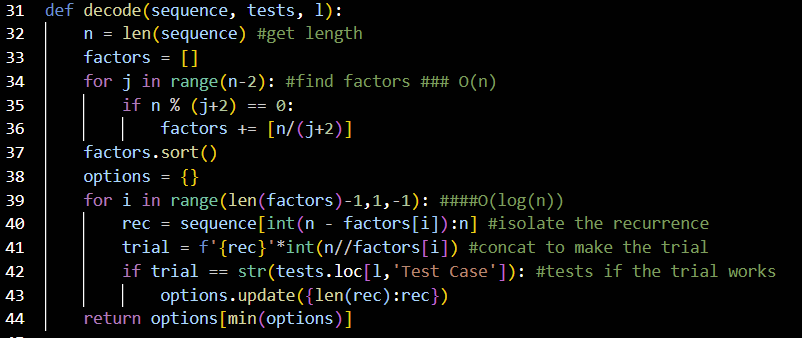
\includegraphics[width=1\linewidth]{Decoding.png}
    \caption{Algorithm Implementation}
    \label{fig:placeholder}
\end{figure}
\vspace{11in}

\subsection{Efficiency Results}
The coefficient of our time complexity is shown to converge for $O(n+\log(n))$ as follows.
\begin{figure}[H]
    \centering
    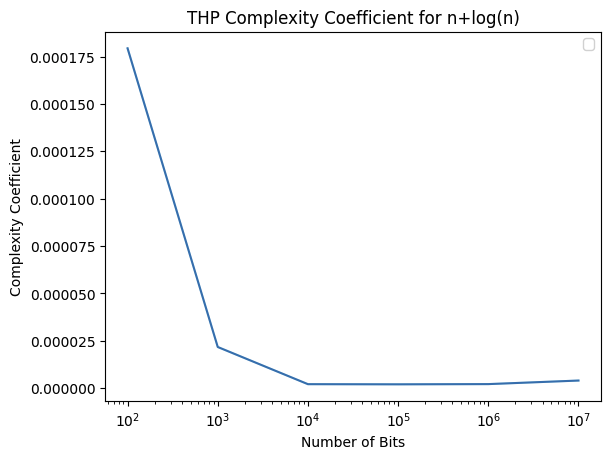
\includegraphics[width=0.7\linewidth]{complexityCoeff}
    \caption{Convergence to Complexity Coefficient}
    \label{fig:placeholder}
\end{figure}
$\newline$
The associated graph of computation time (in seconds) is as follows.
\begin{figure}[H]
    \centering
    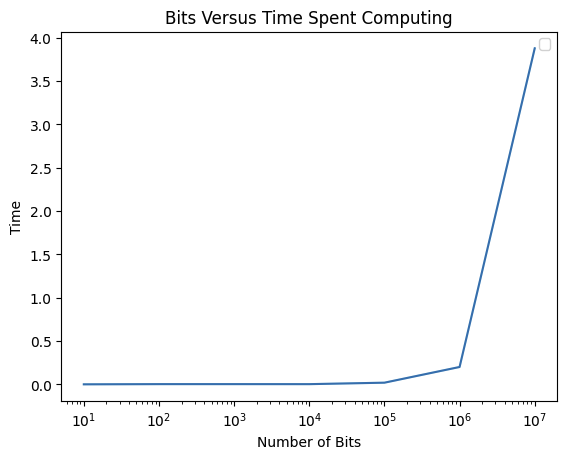
\includegraphics[width=0.7\linewidth]{timeComp.png}
    \caption{Our Results}
    \label{fig:placeholder}
\end{figure}
$\newline$
The jump to $4$ seconds seems extreme, but when we compare it to the Berlekamp-Massey algorithm for the same number of bits, it really doesn't seem bad at all!
\begin{figure}[H]
    \centering
    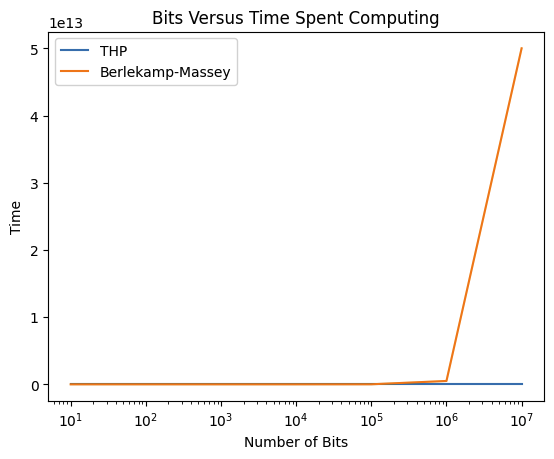
\includegraphics[width=0.7\linewidth]{bmComp.png}
    \caption{Our Results (Compared to Berlekamp Massey)}
    \label{fig:placeholder}
\end{figure}

\subsubsection{Differences From the Berlekamp-Massey Framework}
While the Berlekamp-Massey algorithm can work with partial strings, an admitted hurdle for the use of the Tarter-Herasymov-Priebracha algorithm is that it requires full strings of ciphertext for a combinatorial attack to work. Additionally, the Berlekamp-Massey algorithm provides the recurrence polynomial which provides the recurrence - the THP algorithm provides the recurrence from which the recurrence polynomial can be derived. This mutual inverse property is ultimately irrelevant to the application of either algorithm to a problem. 

$\newline$The Berlekamp-Massey algorithm will work better when an LFSR sequence does not encounter additional noise in transmission between senders and receivers whereas the THP algorithm requires perfect information of the intended LFSR ciphertext. 

$\newline$Ultimately, both algorithms have their optimal use cases; the authors of this paper recommend the THP algorithm for instances where LFSR sequences are perfectly received but have computationally infeasible lengths. 

\vspace{11in}

\section*{Works Cited}

$\newline$
Galbraith, S. D. (2007). Cryptography and coding: 11th IMA International Conference, Cirencester, UK, December 18-20, 2007: Proceedings. Springer. 

$\newline$
Guibas, L. J., \& Odlyzko, A. M. (1981). Periods in strings. Journal of Combinatorial Theory, Series A, 30(1), 19–42. https://doi.org/10.1016/0097-3165(81)90038-8 

$\newline$
Kreczmar, A., \& Mirkowska, G. (1989). Mathematical Foundations of Computer Science 1989: Porabka-Kozubnik, Poland August 28 - September 1, 1989 proceedings. Springer-Verlag: Springer e-books. 

$\newline$
Nikolaev, S. (2025). Advanced berlekamp–Massey method as a basis for finding periodicities in bitstreams. Cybernetics and Systems Analysis, 61(1), 3–10. https://doi.org/10.1007/s10559-025-00739-1 

$\newline$
Tomlinson, M., Tjhai, C. J., Ambroze, M. A., Ahmed, M., \& Jibril, M. (2017). Error-correction coding and decoding bounds, codes, decoders, analysis and applications. Springer International Publishing. 

$\newline$
Wu, Y. (2023). High-speed LFSR decoder architectures for BCH and GII codes. IEEE Journal on Selected Areas in Information Theory, 4, 331–350. https://doi.org/10.1109/jsait.2023.3304235 

$\newline$
Yu, K., \& Hung, L. (1995). On binary recurrence sequences. Indagationes Mathematicae, 6(3), 341–354. https://doi.org/10.1016/0019-3577(95)93201-k 
\end{document}
